\message{ !name(ro.tex)}\documentclass[a4paper,12pt, oneside]{book}

% \usepackage{fullpage}
\usepackage[italian]{babel}
\usepackage[utf8]{inputenc}
\usepackage{amssymb}
\usepackage{amsthm}
\usepackage{graphics}
\usepackage{amsfonts}
\usepackage{listings}
\usepackage{amsmath}
\usepackage{amstext}
\usepackage{engrec}
\usepackage{rotating}
\usepackage[safe,extra]{tipa}
\usepackage{showkeys}
\usepackage{multirow}
\usepackage{hyperref}
\usepackage{microtype}
\usepackage{enumerate}
\usepackage{braket}
\usepackage{marginnote}
\usepackage{pgfplots}
\usepackage{cancel}
\usepackage{polynom}
\usepackage{booktabs}
\usepackage{enumitem}
\usepackage{framed}
\usepackage{pdfpages}
\usepackage{pgfplots}
\usepackage[cache=false]{minted}
\usepackage{tikz}
\usetikzlibrary{automata,positioning}

\usepackage{tikz}\usetikzlibrary{er}\tikzset{multi  attribute /.style={attribute ,double  distance =1.5pt}}\tikzset{derived  attribute /.style={attribute ,dashed}}\tikzset{total /.style={double  distance =1.5pt}}\tikzset{every  entity /.style={draw=orange , fill=orange!20}}\tikzset{every  attribute /.style={draw=MediumPurple1, fill=MediumPurple1!20}}\tikzset{every  relationship /.style={draw=Chartreuse2, fill=Chartreuse2!20}}\newcommand{\key}[1]{\underline{#1}}

\usepackage{fancyhdr}
\pagestyle{fancy}
\fancyhead[LE,RO]{\slshape \rightmark}
\fancyhead[LO,RE]{\slshape \leftmark}
\fancyfoot[C]{\thepage}



\title{Ricerca Operativa e Pianificazione delle Risorse}
\author{UniShare\\\\Davide Cozzi\\\href{https://t.me/dlcgold}{@dlcgold}\\\\Gabriele De Rosa\\\href{https://t.me/derogab}{@derogab} \\\\Federica Di Lauro\\\href{https://t.me/f_dila}{@f\textunderscore dila}}
\date{}

\pgfplotsset{compat=1.13}
\begin{document}

\message{ !name(ro.tex) !offset(-3) }

\maketitle

\definecolor{shadecolor}{gray}{0.80}
\setlist{leftmargin = 2cm}
\newtheorem{teorema}{Teorema}
\newtheorem{definizione}{Definizione}
\newtheorem{esempio}{Esempio}
\newtheorem{corollario}{Corollario}
\newtheorem{lemma}{Lemma}
\newtheorem{osservazione}{Osservazione}
\newtheorem{nota}{Nota}
\newtheorem{esercizio}{Esercizio}
\tableofcontents
\renewcommand{\chaptermark}[1]{%
  \markboth{\chaptername
    \ \thechapter.\ #1}{}}
\renewcommand{\sectionmark}[1]{\markright{\thesection.\ #1}}
\chapter{Introduzione}
\textbf{Questi appunti sono presi a lezione. Per quanto sia stata
  fatta una revisione è altamente probabile (praticamente certo)
  che possano contenere errori, sia di stampa che di vero e proprio
  contenuto. Per eventuali proposte di correzione effettuare una
  pull request. Link: } \url{https://github.com/dlcgold/Appunti}.\\
\textbf{Grazie mille e buono studio!}\\
\textbf{Immagini tratte dalle slide del corso, docente V. Messina}
\chapter{Introduzione alla Ricerca Operativa}
La\textbf{ Ricerca Operativa} è essenziale nel \textit{problem
  solving} e nell'ambito del \textit{decision making}.
Sostanzialmente quindi si studia l'ottimizzazione, massimizzando le
performances, l'accuratezza dei costi etc$\ldots$ per raggiungere un
obiettivo. \\ \textit{Sulle slides ci sono vari esempi introduttivi di
  vita reale}\\
Un altro problema studiato dalla riceca operativa sono le previsioni,
mediante algoritmi predittivi che studiano i \textit{pesi} delle
osservazioni (cosa utile nel \textbf{Machine Learning} in quanto sono
un uso di base delle \textbf{Reti Neurali}, \textit{vari esempi
  introduttivi sulle slides}).\\
\textbf{La ricerca operativa si occupa di formalizzare un problema in
  un modello matematico e calcolare una soluzione ottimo o
  approssimata}. Essa costituisce un approccio scientifico alla
risoluzione di problemi complessi da ricondurre alla matematica
applicata. È utile in ambiti economici, logistici, di progettazione di
servizi e di sistemi di trasporto e, ovviamente, nelle tecnologie.
\textit{È la branca della matematica più applicata}.\\
Il \textit{primo passo} consiste nel costruire un modello traducendo il
problema reale in linguaggio anturale in un linguaggio matematico, che
non è ambiguo. Il \textit{secondo passo} consiste nella costruzione delle
soluzioni del modello tramite algoritmi e programmi di calcolo. Il
\textit{terzo passo}, ovvero l'ultimo, è l'interpretazione e la
valutazione delle soluzioni del modello rispetto a quelle del problema
reale.\\
La ricerca operativa ha origini nel 1800 in un ambiente puramente
matematico. È stata resa ``\textit{algoritmica}'' con la Macchina di
Turing. \textbf{La ricerca operativa usa anche tecniche numeriche e
  non solo analitiche}.\\
Negli ultimi hanno si sono sviluppati, mediante il concetto di
\textbf{gradiente}, nuovi algoritmi per il \textbf{deep network}.\\
\section{Modelli nella R.O.}
\begin{definizione}
  Data una funzione $f:\mathbb{R} \to mathbb{R}$ e $X\subseteq
  \mathbb{R}^n$ un \textbf{problema di ottimizzazione} può esssere
  formulato come:
  \[opt\,\,f(x)\,\,s.t. \,\,x\in X\]
  dove con $opt={\min, \max}$ indendiamo che opt può essere o min o max,
  portando ad un problema di minimizzazione con $\min\,f(x)$ o di
  massimizzazione $\max\,f(x)$. \\
  $f(x)$ è detta \textbf{funzione obiettivo} e vale che:
  \[max[f(x):\,x\in X] = -min[-f(x):\,x\in X]\]
  Inoltre $x\subseteq\mathbb{R}^n$ è \textbf{l'insieme delle soluzioni
    ottenibili} o anche \textbf{regione ammissibile}.\\
  Infine $x\in X$ rappresenta il \textbf{vettore delle variabili
    decisionali} e si tratta di variabili numeriche i cui valori
  rappresentano la soluzione del problema. \\
  \textbf{Si capisce che essendo in $\mathbb{R}$ si hanno infinite
    soluzioni}.\\
  \textbf{Quindi, un problema di ottimizzazione consiste nel
    determinare, se esiste, un punto di minimo/massimo della
    funzione $f$ tra i punti dell’insieme $X$}
  Se $X=\mathbb{R}^n$ si ha un'\textbf{ottimizzazione non vincolata},
  altrimenti, $x\subset \mathbb{R}$ si ha un'\textbf{ottimizzazione
    vincolata}, dove la ricerca dei punti di ottimo della funzione
  obiettivo è fatta su un sottoinsieme proprio dello spazio di
  definizione tenendo però conto dei vincoli. Se ho una funzione
  obiettivo lineare non si può avere un'ottimizzazione non vincolata
  (non saprei cercare massimi e minimi senza vincoli).\\
  Abbiamo poi l'\textbf{ottimizzazione intera o a numeri interi}
  se $x\in \mathbb{Z}^n$ e si possono avere ottimizzazioni miste se si
  hanno interi e reali. Si ha anche l'\textbf{ottimizzazione binaria}
  quando si hanno due vie decisionali. \\
  \textbf{Se non specificato si intende $X\subseteq\mathbb{R}}$.
\end{definizione}
\begin{definizione}
  Quando l'insieme $X$ delle soluzioni ammissibili di un problema di
  ottimizzazione è espresso in un sistema di equazioni o disequazioni si
  parla di \textbf{problema di programmazione matematica (PM)}.\\
  Come vincolo si ha un'espressione $g_i(x)\{\leq, =, \geq\} 0$
  ($g_i\geq 0$ etc $\ldots$) e con
  $g_i:X\to \mathbb{R}$ che è una generica funzione che lega due
  variabili. \\
  \textbf{Si possono avere più vincoli ma si ha sempre l'uguale in ogni
    vincolo per permettere il funzionamento degli algoritmi}.\\
  La regione ammissibile è $X\subseteq\mathbb{R}^n$ che è l'intersezione
  di tutti i vincoli del problema
  \[X=\{x\in\mathbb{R}^n|\, g_i(x)\{\leq, 0, \geq\}0,\,i=1,\ldots,m\]
  Si hanno quindi $m$ vincoli e $n$ variabili.
  \textbf{Se $x \in X$ allora $x$ è soluzione ammissibile,
    se $x \not\in X$ allora $x$ è non ammissibile}
\end{definizione}
\begin{esempio}
  abbiamo la funzione obiettivo
  \[\min_{x,y}(x^2+y^2)\]
  con i 3 vincoli:
  \[x+y \leq 3\]
  \[x\geq 0\]
  \[y\geq 0\]
  la regione ammissibile è:
  \[\{x\in\mathbb{R}^2|\,x+y \leq 3,\,\,x\geq 0,\,\,y\geq 0\}\]
  ovvero l'area sottesa alla retta e compresa negli assi cartesiani:
  \begin{center}
    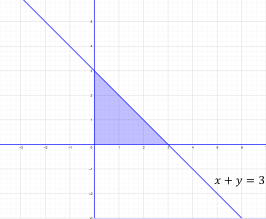
\includegraphics[scale = ]{img/tri.png}
  \end{center}
\end{esempio}
Si possono avere problemi con regione non ammissibile, ovvero con
$X=\emptyset$, che implica che il problema è mal posto oppure bisogna
abbassare qualche vincolo. Si può avere un problema illimitato con:
\[\forall c \in \mathbb{R}\exists x_c\in X:f(x_c)\leq c\,\, se\,\,
  opt = min\]
\[\forall c \in \mathbb{R}\exists x_c\in X:f(x_c)\geq c\,\, se\,\,
  opt = max\]
Infine si può avere una sola soluzione ottima o più (anche infinite)
soluzioni ottime utte con lo stesso valore della funzione
obiettivo.
\begin{esempio}
  abbiamo la funzione obiettivo
  \[\min_{x,y}(x^2+y^2)\]
  con i 3 vincoli:
  \[x+y \leq -1\]
  \[x\geq 0\]
  \[y\geq 0\]
  Non ha soluzione (è matematicamente impossibile) e il problema
  non è ammissibile
\end{esempio}
\begin{esempio}
  abbiamo la funzione obiettivo
  \[\max_{x,y}(x^2+y^2)\]
  con i 2 vincoli:
  \[x\geq 0\]
  \[y\geq 0\]
  Ha come soluzione infinito
\end{esempio}
\begin{esempio}
  abbiamo la funzione obiettivo
  \[\max_{x,y,z}(z)\]
  con i 4 vincoli:
  \[x+y+z = 2\]
  \[0\leq x \leq 1\]
  \[0\leq y \leq 1\]
  \[0\leq z \leq 1\]
  Ha infinite soluzioni (tutte le soluzioni con $z=1$ e $x+y=1$, in quanto cerco
  il max di z e come ultio vincolo ho che al massimo è 1)
  \begin{center}
    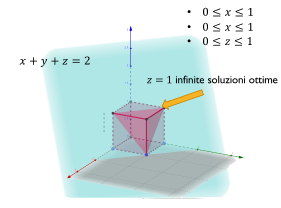
\includegraphics[scale = 1]{img/tri2.png}
  \end{center}
\end{esempio}
La risoluzione di un problema di Programmazione matematica consiste
nel trovare una soluzione ammissibile che sia un \textbf{ottimo
  globale} ovvero un vettore $^*\in X$ tale che:
\[f(x^*)\leq f(x)\,\,\forall x\in X\,\,se\,\,opt=\min\]
\[f(x^*)\geq f(x)\,\,\forall x\in X\,\,se\,\,opt=\max\]
Quando il problema è molto difficile da risolvere possiamo
accontentarci di un ottimo locale, vale a dire un $\hat{x}\in X$ tale
che, fissato un $\varepsilon > 0$ opportuno si ha che (per problemi di
minimo e massimo):
\[f(\hat{x})\leq f(x)\,\,\forall x\in X:\,\||x-\hat{x}||\leq
  \varepsilon\,\,se\,\,opt=\min\]
\[f(\hat{x})\geq f(x)\,\,\forall x\in X:\,\||x-\hat{x}||\leq \varepsilon\,\,se\,\,opt=\max\]
Un problema di ottimizzazione può avere più ottimi locali e globali e
i punti di ottimo globale sono anche di ottimo locale.
\begin{center}
  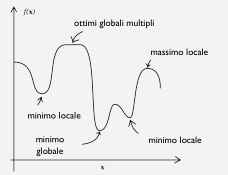
\includegraphics[scale = 1.3]{img/opt.png}
\end{center}
\newpage
\begin{esempio}
  abbiamo la funzione obiettivo:
  \[\min_{x,y}((x-0.2)^2+y^2)\]
  con i 3 vincoli:
  \[x+y \leq 1\]
  \[x\geq 0\]
  \[y\geq 0\]
  In viola si ha la funzione obiettivo tridimensionale e convessa
  e in azzurro la regione ammissibile
  \begin{center}
    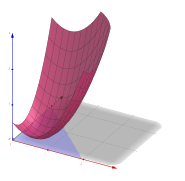
\includegraphics[scale = 1.3]{img/optes.png}
  \end{center}
  si ha solo un minimo globale.
  Si possono usare le \textbf{curve di livello} che sono le proiezioni
  ortogonali sul piano cartesiano ottenute intersecando il piano z con
  il grafico della funzione.\\
  In generale si useranno tecniche numeriche anche se si ha che
  \textbf{una funzione convessa ha un solo minimo globale}
\end{esempio}
\newpage
\begin{esempio}
  abbiamo la funzione obiettivo:
  \[\min_{x}(0.2x^2+(1-\cos(\pi x)))\]
  con i 2 vincoli:
  \[x\geq 5\]
  \[y\geq 0\]
  e si ha il seguente grafico:
  \begin{center}
    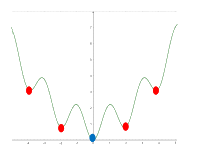
\includegraphics[scale = 1.3]{img/optes2.png}
  \end{center}
  si ha il coseno quindi si ha una funzione nè concava nè convessa
  si ha quindi un ottimo globale e 4 locali
\end{esempio}
Si ha:
\begin{itemize}
  \item \textbf{programmazione lineare (PL)}, con obiettivo e vincoli
  lineari:
  \[opt\,f(x)=c^T x\]
  \[X=\{x\in\mathbb{R}^n:\, g_i(x)\{\leq, =, \geq\}0,\,\,
    i=1,\ldotsm\,\, g_i(x)=a_i^T x-b_i\}\]
  \item \textbf{programmazione lineare intera (PLI)}, con obiettivo e
  vincoli lineari interi:
  \[opt\,f(x)=c^T x\]
  \[X=\{x\in\mathbb{Z}^n:\, g_i(x)\{\leq, =, \geq\}0,\,\,
    i=1,\ldotsm\,\, g_i(x)=a_i^T x-b_i\}\]
  \item \textbf{programmazione non lineare (PNL)}, con obiettivo e
  vincoli $g_i(x)$ non lineari:
  \[opt\,f(x)\]
  \[X=\{x\in\mathbb{R}^n:\, g_i(x)\{\leq, =, \geq\}0,\,\,
    i=1,\ldotsm\,\, g_i(x)=a_i^T x-b_i\}\]
\end{itemize}
\begin{esempio}
  abbiamo la funzione obiettivo:
  \[\min_{x,y}(x^2+y^2)\]
  con i 3 vincoli:
  \[x+y\leq 1\]
  \[x\geq 0\]
  \[y\geq 0\]
  non è lineare in quanto x e y sono al quadrato e quindi non lineare
\end{esempio}
\begin{esempio}
  abbiamo la funzione obiettivo:
  \[\min_{x,y}(x+y)\]
  con i 2 vincoli:
  \[x^2-1\geq 0\]
  \[y\geq 0\]
  non è lineare in quanto ho un vincolo al quadrato e quindi non
  lineare 
\end{esempio}
\begin{esempio}
  abbiamo la funzione obiettivo:
  \[\min_{x,y}(x+4y)\]
  con i 4 vincoli:
  \[x+y=3\]
  \[x^2-1\geq 0\]
  \[x\geq 0\]
  \[y\geq 0\]
  non è lineare in quanto ho un vincolo al quadrato e quindi non
  lineare ma posso renderlo lineare in quanto $x^2-1=(x-1)(x+1)$ ma
  $x+1$ è sempre positivo quindi posso ammorbidire il vincolo
  rendendo il problema lineare
\end{esempio}
\begin{esempio}
  \begin{center}
    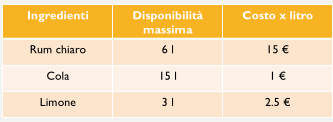
\includegraphics[scale = 0.7]{img/cub.png}
  \end{center}
  Le dosi ideali sono: almeno il 25\% di rum (R) chiaro e il 50\% di
  Cola (C) e non più del 10\% di limone (L) e voglio 10L di cubalibre. Abbiamo quindi, per logica:
  \[R\geq 0\]
  \[C\geq 0\]
  \[L\geq 0\]
  \[R\leq 6\]
  \[C\leq 15\]
  \[L\leq 3\]
  quindi:
  \[0\leq R\leq 6\]
  \[0\leq C\leq 15\]
  \[0\leq L\leq 3\]
  inoltre:
  \[R+C+L\geq 10\]
  che è:
  \[R+C+L -10\geq 0 = \left[
      \begin{matrix}
        1 & 1 & 1
      \end{matrix}
    \right]\left[
      \begin{matrix}
        R \\
        C \\
        L
      \end{matrix}
    \right] -10 \geq 0\]
  quindi:
  \[a_1^T= \left[
      \begin{matrix}
        1 & 1 & 1
      \end{matrix}
    \right], \,x =\left[
      \begin{matrix}
        R \\
        C \\
        L
      \end{matrix}
    \right],\, b_1=10 \]
  Cosa vuol dire almeno il 25\% di rum chiaro?
  \[R \geq 0.25 \cdot (R + C + L)\]
  Cosa vuol dire almeno il 5o\% di cola?
  \[R \geq 0.5 \cdot (R + C + L)\]
  Cosa vuol dire almeno il 25\% di limone?
  \[R \geq 0.1\cdot (R + C + L)\]
  che sono vincoli lineari.\\
  quindi il costo è:
  \[\min_{R,C,L}(15R+C+2.5L)\]
  che è una funzione obiettivo lineare.\
  Osserviamo che la funzione obiettivo può essere scritta anche nella
  seguente forma compatta:
  \[\min c^tx,\,\con\,\,c^t=\left[
      \begin{matrix}
        15 & 1 & 2.5
      \end{matrix}
    \right]\,\,e\,\, x =\left[
      \begin{matrix}
        R \\
        C \\
        L
      \end{matrix}
    \right] \]
  Ora riscriviamo in forma matriciale:
  \[\min cx\]
  \[Ax\geq b\]
  \[x\geq 0\]
  con:
  \[c=\left[
      \begin{matrix}
        15 & 1 & 2.5
      \end{matrix}
    \right]\]
  \[x =\left[
      \begin{matrix}
        R \\
        C \\
        L
      \end{matrix}
    \right]\]
  la prima riga sarà $R+C+L\geq 10$\\
  la seconda sarà $R\geq 0.25\cdot (R+C+L) \geq 0 \to
  (1-0.25)R-0.25R-0.25L$\\
  la terza sarà $C\geq 0.5\cdot (R+C+L) \geq 0 \to
  -0.5R + (1-0.5)C-0.5L$\\
  la quarta sarà $L\geq 0.1\cdot (R+C+L) \geq 0 \to
  -0.1R -0.25C +0.9(1-0.1)L$\\
  la quinta sarà $0 \leq R \leq 6 \to -R \geq -6$\\
  la sesta sarà $0 \leq C \leq 15 \to -C \geq -6$\\
  la settima sarà $0 \leq L \leq 3 \to -L \geq -6$\\
  e quindi:
  \[Ax=\left[
      \begin{matrix}
        1 & 1 & 1 \\
        0.75 & -0.25 & -0.25 \\
        -0.5 & 0.5 & -.5 \\
        0.1 & 0.1 & -0.9 \\
        -1 & 0 & 0 \\
        0 & -1 & 0 \\
        0 & 0 & -1
      \end{matrix}
    \right]
    \left[
      \begin{matrix}
        R \\
        C \\
        L
      \end{matrix}
    \right] \geq
    \left[
      \begin{matrix}
        10 \\
        0 \\
        0 \\
        0 \\
        -6 \\
        -15 \\
        -3 
      \end{matrix}
    \right]\]
\end{esempio}

\begin{esempio}
  Si ha che:
  \begin{center}
    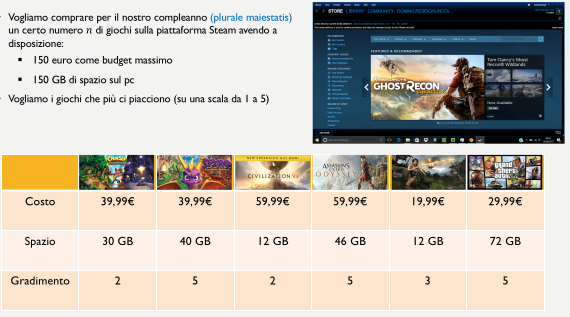
\includegraphics[scale = 0.7]{img/steam.png}
  \end{center}
  Il comprare o no un videogioco può essere modellizzato per mezzo
  di variabili decisionali binarie associate ad ogni gioco usando
  variabili binarie:
  \[x_i\in\{0,1\}\,i=1,\ldots n\]
  con $x_i=1$ si compra con $x_i=0$ no.\\
  Non superare il budget massimo di 100 euro può essere espresso
  dalla seguente relazione:
  \[39,99 \cdot x_1 + 39,99 \cdot x_2 + 59,99 \cdot x_3 + 59,99 \cdot
    x_5 + 19,99 \cdot x_5+ 29,99 \cdot x_6 ≤ 150\]
  Non superare la memoria massima può essere espresso dalla seguente
  relazione:
  \[30 \cdot x_1 + 40 \cdot x_2 + 12 \cdot x_3 + 46 \cdot
    x_5 + 12 \cdot x_5+ 70 \cdot x_6 ≤ 150\]
  e sono vincoli lineari.\\
  Volere i giochi che più ci piacciono si esprime nel seguente modo:
  \[\max(2\cdot x_1+5\cdot x_2+2\cdot x_3+5\cdot x_4+3\cdot x_5+5\cdot x_6)\]
  che è una funzione obiettivo lineare.\\
  Volere i giochi che più ci piacciono, avendo 200 euro di budget e
  100GB si spazio corrisponde a:
  \[\max(2\cdot x_1+5\cdot x_2+2\cdot x_3+5\cdot x_4+3\cdot x_5+5\cdot x_6)\]
  \textbf{Si tratta, quindi, di un problema di programmazione lineare a
    variabili binarie, che sono un caso particolare di variabili
    intere}.\\
  \textbf{\textit{Un modello di ottimizzazione di questo tipo prende
      il nome di Problema dello zaino (Knapsack)}}
\end{esempio}
\textbf{altri esempi sulle slide}
\begin{esempio}
Partendo dai dati di vendita di avatar capire se Endgame supererà gli
incassi di avaatar, sapendo gli incassi dei primi giorni.\\
Vogliamo costruire una retta di regressione lineare che interpoli i
dati:
\[y=ax+b,\,\,a,b\in\mathbb{R}\]
Bisogna calcolare la retta di regressione corrisponde al seguente problema di
ottimizzazione non vincolata:
\[\min_{a,b}\left[\frac{1}{2}\sum_{i=1}^n (y_i-ax_i-b)^2\right]\]
e quindi si ha funzione obiettivo non-lineare con $a,b$ variabili
continue. Cerco quindi la retta di regressione partendo dai primi dati
e ipotizzo una previsione e cerco $a$ e $b$
:
\begin{center}
  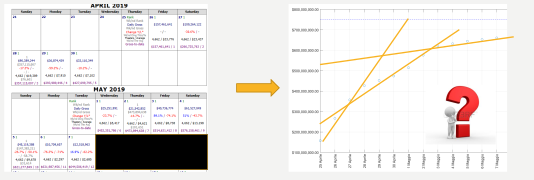
\includegraphics[scale = 0.9]{img/prev.png}
\end{center}

\begin{center}
  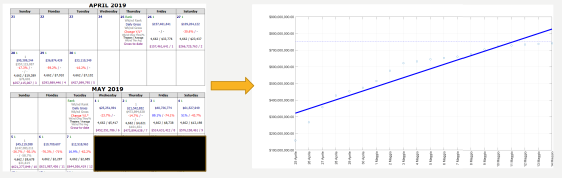
\includegraphics[scale = 0.9]{img/prev2.png}
\end{center}
\textbf{Questo è un problema di ottimizzazione non vincolata e non lineare}
\end{esempio}
\textbf{altri esempi sulle slide}
\subsection{Esercizio}
\begin{esercizio}
  \textbf{testo:}\\
  \textit{La Svivon produce  batterie  elettriche  di  tre  tipi
    (Alfa,  Beta  e  Gamma).  Per  due  di  esse  (Beta  e  Gamma)
    utilizza del rame. Per coprire la produzione del prossimo mese, può
    acquistare il rame al prezzo di 5 euro/kg. Il fornitore però non
    può fornire più di 4000  kg  di rame.  Nella  seguente  tabella
    sono  indicate: la  quantità di  rame  richiesta  per  ciascuna
    batteria, i costi di manodopera (per batteria prodotta) e prezzi
    di vendita al pubblico (per batteria):}
  \begin{center}
    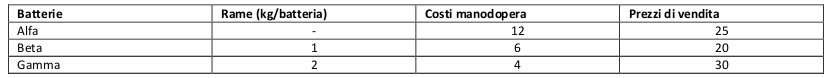
\includegraphics[scale = 0.7]{img/es1.png}
  \end{center}
  \textbf{(costi e manodopera sono entrambi in euro/batteria)}\\
  \textbf{Si suppinga che ogni batteria prodotta sia anche venduta.}\\
  \textit{I tre tipi di batteria vogliono essere prodotti in quantità
    tali che il numero di batterie di tipo Alfa sia almeno doppio del
    numero  di  batterie  di  tipo  Beta  e  non  superiore  al
    numero di  batterie  Gamma.  Formulare un  opportuno  modello
    di programmazione lineare per la pianificazione ottimale
    dell’attività diproduzione della Svivon.}\\
  \textbf{Soluzione:}\\
  Innazitutto partiamo dal'ultima frase e definiamo le relazioni tra i
  tipi di batteria. Definiamo $x_i$ il numero di batterie di tipo
  $i\in I$, con   $I=\{\alpha, \beta, \gamma\}$ \textbf{insieme degli
    indici}. Cerchiamo ora funzione \textbf{obiettivo} e
  \textbf{vincoli}.\\
  Suppongo di produrre una batteria di tipo $\alpha$, avrò un guadagno
  effettivo pari a guadagno meno costi: $25-12=13$. Per le $\beta$ si
  avrà, avendo anche il costo del rame di 5 euro al kilo, $20-6-5\cdot
  1= 9$. Per le $\gamma$ sarà $30-4-5\cdot 2 = 16$. L'azienda
  ovviamente vuole guadagnare di più, dobbiamo massimizzare il
  profitto. Il profitto delle $\alpha$ sarà $13x_\alpha$, per le
  $\beta$ sarà $9x_\beta$ e per le $\gamma$ sarà $16x_\gamma$.
  Quindi si avrà la seguente funzione obiettivo:
  \[\max(z) = 13x_\alpha+ 9x_\beta +16x_\gamma\]
  con i seguenti vincoli (ricordando che solo le $\beta$ e le $\gamma$
  usano il rame):
  \[
    \begin{cases}
      x_\alpha \geq 2x_\beta \\
      x_\alpha \leq x_\gamma \\
      x_\beta +2x_\gamma < 4000
    \end{cases}
  \]
  Bisogna specificare che le variabili non sono continue, quindi
  aggiungiamo un vincolo di interezza:
  \[x_i\in\mathbb{N},\, \forall i\in I\]
  E abbiamo risolto le richieste dell'esercizio
\end{esercizio}
\begin{esercizio}
  \textbf{Testo:}\\
  \textit{Un’industria con dueimpianti  produttivi  localizzati  a
    Rimini e Firenze è interessata a sapere qual è l’organizzazione
    ottimale della propria rete distributiva, in modo da ottimizzare
    la consegna dei prodotti presso letreprincipali città di
    distribuzione:Palermo, Milano  e Roma.  La  capacità  produttiva
    dei  due  impianti  di  produzione  è  la  seguente: Rimini 300,
    Firenze 600. La domanda presso le tre città di distribuzione è
    la seguente: Palermo 325, Milano 300, Roma 275. I costi associati
    al viaggio tra gli impianti di produzione e le città di
    distribuzione sono dati dalla seguente tabella:}
  \begin{center}
    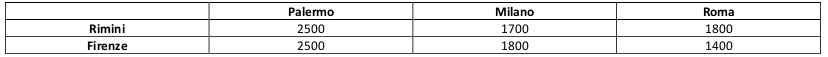
\includegraphics[scale = 0.7]{img/es3.png}
  \end{center}
  \textit{Formulare un modello di Programmazione lineare che
    permetta di pianificare lo spostamento ottimale dei prodotti
    dagli impiantialle cittàdi distribuzione in modo tale da
    minimizzare i costi di viaggio}\newpage
  \textbf{Soluzione:}\\
  \begin{center}
  \begin{tikzpicture}[shorten >=1pt,node distance=7cm,on grid,auto]
    \node[state] (q_0)   {$RN (300)$};
    \node[state] (q_1) [above right =of q_0] {$PA(-325)$};
    \node[state] (q_2) [below=of q_0] {$FI(600)$};
    \node[state] (q_3) [ right =of q_2] {$MI(-300)$};
    \node[state] (q_4) [right =of q_0] {$RM(-275)$};
    \path[->]
    (q_0) edge  node  {$2500$} (q_1)
    (q_0) edge  node  [right = 2pt]{$1700$} (q_3)
    (q_0) edge  node  {$1800$} (q_4)
    (q_2) edge  node  {$2500$} (q_1)
    (q_2) edge  node  {$1800$} (q_3)
    (q_2) edge  node  {$1400$} (q_4);
  \end{tikzpicture}
\end{center}
Sugli archi ho i costi di trasporto.\\
Definisco due insiemi indici, uno $I=\{RN,FI\}$ con le città di
partenza, e uno $J=\{PA, MI, RM\}$ con le città d'arrivo. \\
Quindi le varfiabili $x_{i,j}$ indicano il numero di prodotti
trasportati da dalla città $i\in I$ a quella $j\in J$.\\
Avrò la seguente funzione obiettivo:
\[\min(z)= 2500x_{RN, PA} + 1700x_{RN, MI}+\cdots + 1400x_{FI,RM}\]
che può essere scritta in maniera compatta definendo il dato $c_{i,j}$ come il
costo di trasporto tra le due città $i$ e $j$, ottenendo:
\[\min(z)=\sum_i\sum_jc_{i,j}x_{i,j}\]
Cerchiamo ora i vincoli. A Rimini possono uscire 300 prodotti:
\[x_{RN,PA}+x_{RN,MI}+x_{RN,RM}=300\]
una cosa simile va fatta per Firenze.\\
Per le città di arrivo vediamo l'esempio di Palermo:
\[x_{RN,PA}+x_{FI_PA}=+325\]
similmente per Milano e Roma.\\
Questi vincoli possono essere compattati a livello di sintassi,
indicando con $b_i$ il numero di prodotti spedibili da una città $i\in
I$:
\[\sum_{j\in J}x_{i,j}=b_i,\,\, \forall i \in I\]
e indicando con $b_j$ il numero di prodotti ricevibili da una città
$j\in J$:
\[\sum_{i\in I}x_{i,j}=b_j,\,\,\forall j \in J\]
e aggiungiamo il vincolo per l'interezza:
\[x_{i,j}\in\mathbb{N},\,\,\forall (i,j)\in I\times J\]
\end{esercizio}
\section{Soluzione Grafica}
Consideriamo un problema di programmazione lineare. Abbiamo la
seguente funzione obiettivo:
\[opt\,f(x)=c^Tx\]
con i seguenti vincoli lineari:
\[X=\left{x\in\mathbb{R}^n:\, g_i(x)\{leq, =, \geq\}0,\, i=1\ldots
      m\right}\]
con:
\[g_i(x)=a_i^Tx-b_i,\,\, a\in \mathbb{R}, b\in \mathbb{R}^m,\,\, c\in
  \mathbb{R}^n,\,\,opt=\{min, max\}\]
I problemi di ottimizzazione reali si presentano in forma PL se sono
verificate le seguenti ipotesi:
\begin{itemize}
  \item \textbf{proporzionalità:} il contributo di ogni variabile
  decisionale al valore della funzione obiettivo è proporzionale
  rispetto al valore assunto dalla variabile stessa
  \item \textbf{additività:} ogni funzione è la somma dei contributi
  delle variabili
  \item \textbf{continuità:} qualunque valore delle variabili in
  $\mathbb{R}^n$  è accettabile
\end{itemize}
\begin{shaded}
  Diamo due definizioni:
  \begin{itemize}
    \item in uno spazio euclideo un \textbf{insieme convesso} è un insieme
    nel quale, per ogni coppia di punti, il segmento che li congiunge
    è interamente contenuto nell'insieme
    \begin{center}
      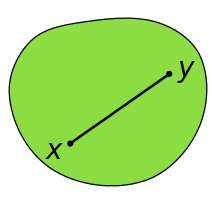
\includegraphics[scale = 0.7]{img/conv.png}
    \end{center}
    \item in uno spazio euclideo un \textbf{insieme non convesso} è un insieme
    nel quale, per ogni coppia di punti, il segmento che li congiunge non
    è interamente contenuto nell'insieme
    \begin{center}
      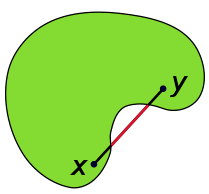
\includegraphics[scale = 0.7]{img/conc.png}
    \end{center}
  \end{itemize}
\end{shaded}
Tornando al problema iniziale iniziamo a studiare il caso
\textbf{2D}. In questo caso si ha che:
\begin{itemize}
  \item i vinvoli $g_i(x)$ possono essere rette (se $g_i(x)=0$) o
  semipiani (se $g_i(x)\neq 0$)
  \item la regione ammissibile $X$ risulta essere un sottoinsieme
  convesso del piano cartesiano
  \item la funzione obiettivo $z=c_1x_1+c_2x_2$ è un piano nello
  spazio $\mathbb{R}^3$
\end{itemize}
\textit{assumiamo inoltre, senza perdere generalità, un vincolo di
  non negatività delle variabili, ovvero $x_1,x_2\geq 0$}.\\
Un vincolo del tipo $a_1x_1+a_2x_2=b_1$ è una retta nel piano, con
l'inclinazione che è perpendicolare al vettore $v=(a_1,a_2)$:
\begin{center}
  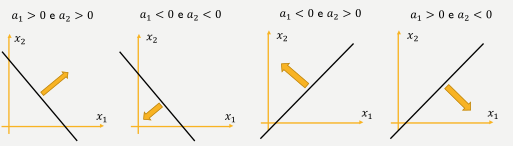
\includegraphics[scale = 0.7]{img/2d.png}
\end{center}
Questo viene detto \textbf{vincolo retta}.\\
Studiamo ora il \textbf{vincolo semipiano}, che è un vincolo del tipo
$a_1x_1+a_2x_2\leq b_1$ (che è appunto un semipiano).
\begin{shaded}
  Per disegnare il semipiano disegnamo prima la retta associata
  $a_1x_1+a_2x_2=b_1$. Scegliamo poi un punto non appartenente a tale
  retta e:
  \begin{itemize}
    \item se il punto verifica la disuguaglianza allora scegliamo il
    semipiano che lo contiene
    \item altrimenti scegliamo un altro semipiano
  \end{itemize}
  \begin{esempio}
    Si ha $x_1+x_2\leq 2$. Disegnamo quindi $x_1+x_2=2$, scegliamo il
    punto $(0,0)$ e, essendo $0+0\leq 2$ abbiamo che il punto soddisfa
    la disequazione e quindi il semipiano contiene $(0,0)$
  \end{esempio}
  \textbf{Un vincolo del tipo $a_1x_1+a_2x_2\geq b_1$ è uguale a
    $-a_1x_1-a_2x_2\leq -b_1$}
\end{shaded}
\textit{La regione ammissibile X è data dall’intersezione dei vari
  vincoli (rette e semipiani)} e quindi, dal punto di vista geometrico
corrisponde ad un \textbf{poliedro convesso} in $\mathbb{R}^2$, e può
essere limitata (\textbf{politopo}) o illimitata
\begin{center}
  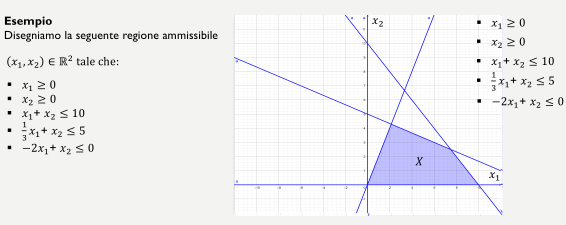
\includegraphics[scale = 0.7]{img/2d1.png}
\end{center}
\begin{center}
  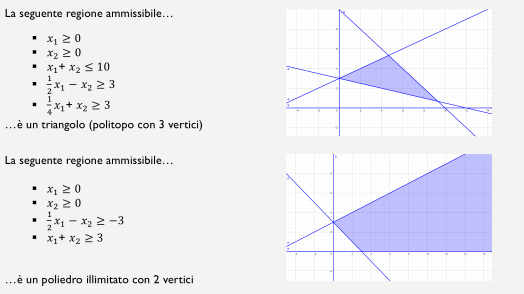
\includegraphics[scale = 0.7]{img/2d2.png}
\end{center}
\begin{esempio}
  Consideriamo il seguente problema di ottimizzazione:
  \[\maz z = -x_1+x_2\]
  con i vincoli:
  \[x_1+x_2\leq 4,\, x_1\geq 0,\, x_2\geq 0\]
  Riscriviamo la funzione obiettivo come $x_2=x_1+z$, che
rappresenta un fascio di rette parallele al variare di $z$, che
all'aumentare si spostano verso il punto $(0,4)$, oltre il quale si
esce dalla regione ammissibile. Quindi la soluzione ottima è il punto
$(0,4)$ che rappresenta un vertice della regione ammissibile (poligono
convesso):
\begin{center}
  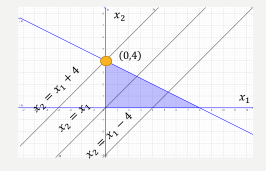
\includegraphics[scale = 0.7]{img/2d3.png}
\end{center}
\end{esempio}
Vediamo il caso 3D.\\
la funzione obiettivo $z=c_1z_1+c_2x_2$ rappresenta un piano nello spazio 3D passante per l’origine
\end{document}
\message{ !name(ro.tex) !offset(-713) }
